\providecommand{\main}{../../..}
\providecommand{\Figures}{\main/Figures}

\documentclass[\main/main.tex]{subfiles}

\begin{document}

\section{\label{sec:sblc}\sblc}

%
%
Du fait de nombreuses étapes de traitements, d'échantillons potentiellement variables, et d'événements perturbateurs comme l'adhérence des échantillons aux parois des tubes ou l'adhérence des échantillons entre eux, les marquages immuno-histochimiques peuvent être de qualité variable. Il est donc souvent compliqué d'optimiser un marquage par anticorps, en particulier pour des expériences dites in toto , impliquant par exemple une larve de \pz{} entière.
%
Les difficultés rencontrées avec le marquage par anticorps anti-HuC/D (qui marque les cellules en neurogenèse de façon complémentaire aux marqueurs lipophiles qui marquent principalement les fibres neuronales)) nous a obligé à mettre au point une procédure de compensation des défauts de marquage.
En partant d'une hypothèse physique simple, nous avons supposé que la concentration de marquage au sein d'un tissu suivait une loin de décroissance exponentielle.
%
L'algorithme de compensation de défaut de marquage
a été nommé \sblc{} (SBLC).
%
Dans la suite de cette section seront présentées les hypothèses, une description de l'algorithme créé, une présentation des résultats obtenus et finalement une discussion des limites de ce procédé.

    \subsection{Hypothèse}
  
%%
%
Dans un tissu fixé, la diffusion des anticorps peut être modélisée 
comme un mouvement brownien.
%
Dans le cadre d'une coupe mince, les anticorps vont circuler dans le milieu environnant le tissu sans contrainte.
%
Une coupe mince de cerveau de poisson-zèbre a une épaisseur comprise entre  2 et 25 µm.
%
La surface est ainsi tellement grande par rapport au volume qu'il est possible de marquer rapidement et uniformément la coupe.

%
Dans le cadre de tissus plus épais, les anticorps vont interagir avec le tissu, et ce dernier va limiter la pénétration de l'anticorps.
%
De manière homologue à la diffusion de la chaleur, on peut alors modéliser la diffusion des anticorps dans le tissu comme une exponentielle décroissante.
%
En partant de ce principe, on peut en déduire que la concentration en anticorps est corrélée à l'épaisseur de tissu traversé.
%
Ainsi, il est parait possible de corriger un défaut de marquage par l'application d'une correction suivant la profondeur des tissus pénétrés par l'anticorps.
%
Les hypothèses posées m'ont donc permis de mettre au point une méthode de correction d'un défaut de marquage immuno-histochimique se basant sur la profondeur de tissus pénétrée par les anticorps.
%
En utilisant une méthode de correction similaire au SBDDCC (voir mansucrit), nous avons ainsi mis au point un algorithme permettant la correction d'un tel défaut de marquage.
    
    \subsection{Algorithme}
 
%%
%
L'obtention de la segmentation de l'échantillon entier est un pré-requis au calcul de cette algorithme.
%
Une manière de réaliser cette segmentation a été présenté en section~\ref{sec:lempereur_info}.

%%
%
La première étape de l'algorithme est le calcul
d'une carte de distance.
%
Cette distance est mesuré depuis la surface de la segmentation.
%
Ainsi, cette carte indiquera le nombre de voxels minimal qu'il faut
traverser pour atteindre chaque voxel au sein de la segmentation.
%
Cette carte va ainsi générer des lignes concentriques au sein de l'échantillon.
%
De cette manière, il est possible de modéliser l'épaisseur de tissus qu'un anticorps a dû traverser avant d'atteindre un point précis.
%

%%
%
En utilisant cette carte, il est alors possible de mesurer la valeur médiane de fluorescence pour chaque épaisseur de tissu.
%
De manière analogue au SBDDCC, on normalise la valeur des médians des valeurs de gris eau médian le plus élevé. Si la profondeur d'une couche est supérieure à la profondeur de la couche ayant le plus grand médian, on multiplie tous les pixels de cette profondeur par le quotient de la valeur médiane maximale et de la valeur médiane de la profondeur de la couche.
%
De cette manière, un défaut de marquage immuno-histochimique 
induisant une perte croissante de l'intensité de la fluorescence avec
l'épaisseur de tissus à pénétrer pour l'anticorps peut être
compensé.

\color{magenta} Mise en équation?\color{black}

%%
%
Afin de visualiser les résultats de cet algorithme, un fantôme théorique a été créé.
%
Pour cela, une ellipse comportant des valeurs de gris 
aléatoirement attribués entre 1 et 4095 a été générée.
%
Cette image est appelé $F$ (voir Figure~\ref{fig:sblc:algo:model}).
%
On conserve les contours de l'ellipse, que l'on considérera par la suite comme la segmentation de l'échantillon (voir Figure~\ref{fig:sblc:algo:ellipse}).
%
On calcule la carte des distances au sein de l'ellipse originelle.
%
Cette carte est appelé appelé $P$ (voir Figure~\ref{fig:sblc:algo:dist}).
%
On va ensuite calculer pour chaque couche un coefficient de décroissance.
%
En prenant pour demi-vie le quart de la profondeur maximale dans l'échantillon (Eq.\eqref{eq:sblc:half}), on calcule alors la valeur d'une exponentielle décroissante pour chaque profondeur (Eq.\eqref{eq:sblc:exp}).
%
Ces coefficients sont alors utilisés pour reproduire l'effet d'une déperdition exponentielle au sein de chaque couche en multipliant les valeurs de gris d'une couche par le coefficient calculé pour cette profondeur (Eq.\eqref{eq:sblc:decay}).
%
De plus, un seuillage est appliqué (Eq.\eqref{eq:sblc:seuillage} pour supprimer les valeurs trop basses dans les zones ayant été dégradées.
%
Le résultat de l'application de cette décroissance exponentielle est visible en Figure\ref{fig:sblc:algo:decay}.

\begin{equation}
    \label{eq:sblc:half}
    t_{1/2} = \frac{max(P)}{4}
\end{equation}

\begin{equation}
    \label{eq:sblc:exp}
    \forall{} e \in \llbracket 1~;~max(P) \rrbracket,~\eta(e) = e^{- t/ t_{1/2}}
\end{equation}

\begin{equation}
    \label{eq:sblc:decay}
    \forall{} x \in I, D(x) =\eta{}(P(x)) * F(x)
\end{equation}

\begin{equation}
    \label{eq:sblc:seuillage}
    \forall{} x \in D, T(x) = 
    \begin{cases}
        D(x), & \text{si } P(x) < \frac{max(P)}{2} \\
        D(x), & \text{si } P(x > \frac{max(P)}{2} \text{ et } D(x) > 10\\
        0, & \text{autrement}
    \end{cases}
\end{equation}

%%
%
L'image ainsi produite est ensuite corrigée en utilisant le \sblc{} (voir Figure~\ref{fig:sblc:algo:correction}).
%
En comparant visuellement le résultat au modèle d'origine, il est difficile d'observer une différence à l'oeil nu.
%
Afin de confirmer cette impression, on a calculé pour chaque voxel le ratio entre le modèle et le résultat de la correction sur l'image dégradée (Eq.\eqref{eq:sblc:ratio}).
%
La visualisation de ce ratio est visible en Figure~\ref{fig:sblc:algo:ratio}.

\begin{equation}
    \label{eq:sblc:ratio}
    \forall x \in F, R(x) = \left| 1 - \frac{T(x)}{F(x)} \right|
\end{equation}

\begin{figure}

    \centering
    \begin{subfigure}[b]{0.30\textwidth}
       \caption{
        \centering
            \label{fig:sblc:algo:model}
            Fantôme
            }
       \centering 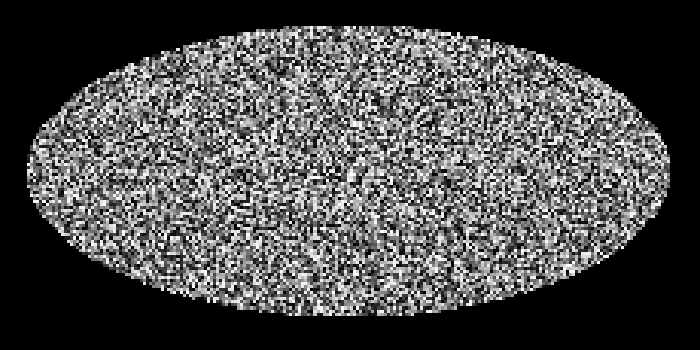
\includegraphics[width=\textwidth]{\Figures/Sblc/model_cut.png}
    \end{subfigure}
    %
    \begin{subfigure}[b]{0.30\textwidth}
       \caption{
        \centering
            \label{fig:sblc:algo:ellipse}
            Ellipse superposée au fantôme
            }
       \centering 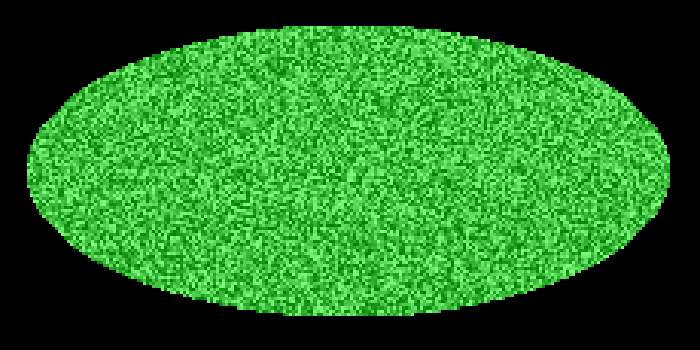
\includegraphics[width=\textwidth]{\Figures/Sblc/ellipse_cut.png}
    \end{subfigure}
    %
    \begin{subfigure}[b]{0.30\textwidth}
       \caption{
        \centering
            \label{fig:sblc:algo:dist}
            Carte des distances
            }
       \centering 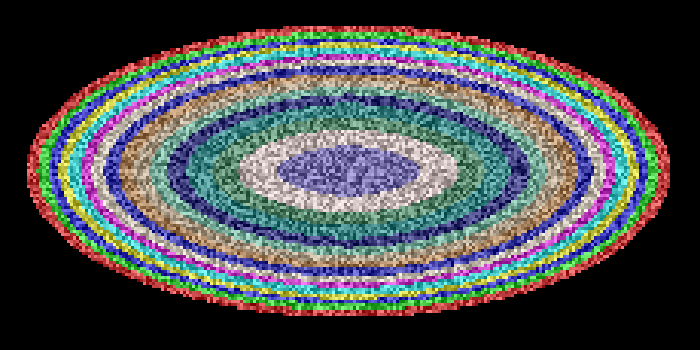
\includegraphics[width=\textwidth]{\Figures/Sblc/dist_cut.png}
    \end{subfigure}
    %
    \begin{subfigure}[b]{0.30\textwidth}
       \caption{
        \centering
            \label{fig:sblc:algo:decay}
            Décroissance exponentielle
            }
       \centering 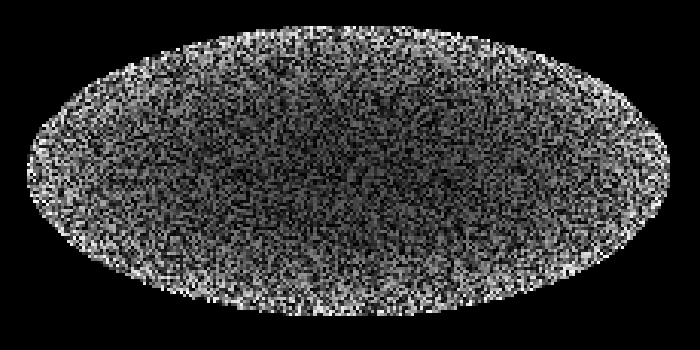
\includegraphics[width=\textwidth]{\Figures/Sblc/decay_cut.png}
    \end{subfigure}
    %
    \begin{subfigure}[b]{0.30\textwidth}
       \caption{
        \centering
            \label{fig:sblc:algo:correction}
            Résultat du SBLC
            }
       \centering 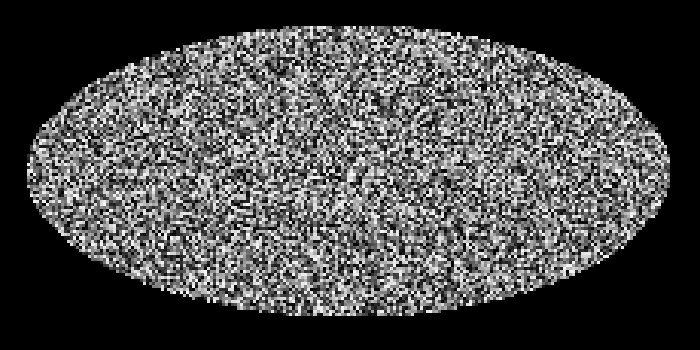
\includegraphics[width=\textwidth]{\Figures/Sblc/correction_cut.png}
    \end{subfigure}
    %
    \begin{subfigure}[b]{0.30\textwidth}
       \caption{
        \centering
            \label{fig:sblc:algo:ratio}
            Ratio des \newline valeurs de gris
            }
       \centering 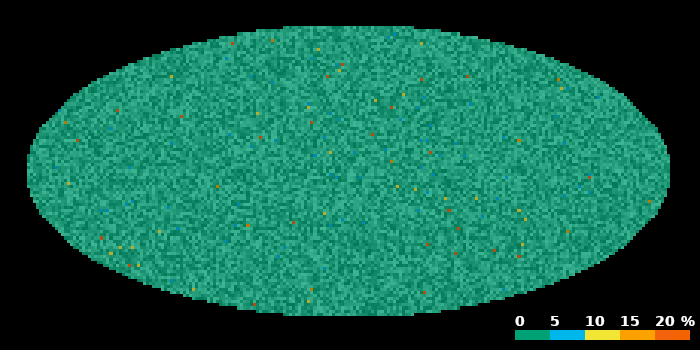
\includegraphics[width=\textwidth]{\Figures/Sblc/delta_cut.png}
    \end{subfigure}
    %
    \caption{
        \label{fig:sblc:algo}
        Illustration du \sblc{} par l'emploi d'un fantôme.
        \newline
        pour créer ce fantôme, on commence par créer l'image de référence,
        puis on lui applique une décroissance exponentielle.
        On applique ensuite le SBLC sur l'image dégradée.
    }
\end{figure}


    \subsection{Résultats et discussions}
    

%%
%
Dans le cadre des marquages \ihc{}, cette approche peut donc permettre de compenser des défauts de pénétration d'anticorps.
%
Certains anticorps, comme anti-HuC/D, présente des gradients de marquages importants.
%
La région marquée ayant une taille importante, il est difficile d'obtenir un marquage homogène sur l'ensemble des tissus (voir Figure~\sec{fig:sblc:huc:raw}).
%
Le SBLC permet ainsi de compenser ce défaut de marquage en corrigeant informatiquement les valeurs de grs. (voir Figure~\ref{fig:sblc:huc:appliqué}).
%
En comparant les deux résultats (Voir Fig~\ref{fig:sblc:huc:comp}), on peut ainsi observer que l'image obtenue n'a eu un effet que dans la profondeur de l'échantillon, et que cet algorithme permet bien de retrouver une information cohérente.

\begin{figure}
    \centering
    \begin{subfigure}[b]{0.30\textwidth}
        
        \caption{image d'origine}
        \centering 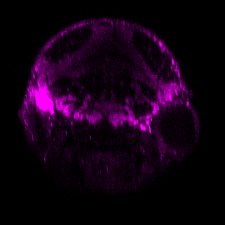
\includegraphics[width=\textwidth]{\Figures/Sblc/huc_original_magenta.png}
        \label{fig:sblc:huc:raw}
    \end{subfigure}
    %
    \begin{subfigure}[b]{0.30\textwidth} 
        \caption{Résultat du SBLC}
        \centering 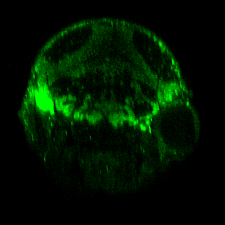
\includegraphics[width=\textwidth]{\Figures/Sblc/huc_corrected_green.png}
        \label{fig:sblc:huc:appliqué}
    \end{subfigure}
    %
    \begin{subfigure}[b]{0.30\textwidth} 
        \caption{superposition}
        \centering 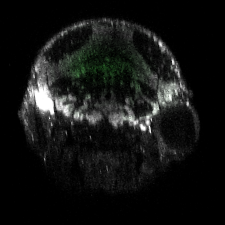
\includegraphics[width=\textwidth]{\Figures/Sblc/huc_compared.png}
        \label{fig:sblc:huc:comp}
    \end{subfigure}
    %
    \caption{
        Résultat de l'application du SBLC représenté par une coupe transversale d'un marquage anti-HuC/D sur un échantillon de \pz{} à 5 dpf.}
    \label{fig:sblc:defaut:surface}
\end{figure}

%%
%
En raison des pré-requis nécessaires à l'emploi de cette méthode, plusieurs limites d'utilisation sont prévisibles.

%%
%
Tout d'abord, cette méthode nécessite que le marquage à corriger soit réparti de façon homogène sur l'ensemble de l'échantillon, ou tout du moins qu'il suive une répartition homogène suivant la profondeur de tissus.
%
L'emploi d'un anticorps marquant une zone limitée dans l'espace pourrait ainsi être problématique, car le signal qui serait amplifié ne serait que du bruit de fond.

%%
%
Pour un exemple plus concret, imaginons un antigène présent uniquement sur la peau du \pz{}.
%
Les anticorps se fixeraient alors sur la peau, ce qui impliquerait une fluorescence induite uniquement sur les couches superficielles de l'échantillon.
%
L'image obtenue serait alors saturée autour de la peau, et quasi-nulle au sein de l'échantillon.
%
Même si l'emploi du SBLC dans ce contexte parait peu adapté, imaginons le résultat de son application sur cette image.
%
Pour les voxels de la peau, les valeurs de gris ne seraient que peu modifié.
%
A l'intérieur de l'échantillon, deux cas de figures apparaissent.
%
Si le voxel à corriger a une valeur nulle, alors l'emploi d'une multiplication n'induira aucun changement.
%
En revanche, si la valeur du voxel est différente de zéro, la normalisation de la valeur de ce voxel lui attribuera une valeur proche des valeurs de gris des régions d'intérêt.
%
L'échantillon se verrait ainsi artificiellement "rempli" par un signal n'existant pas (voir Figure~\ref{fig:sblc:defaut:surface}).

\begin{figure}
    \centering
    \begin{subfigure}[b]{0.45\textwidth}
        
        \caption{Fantôme employé}
        \centering 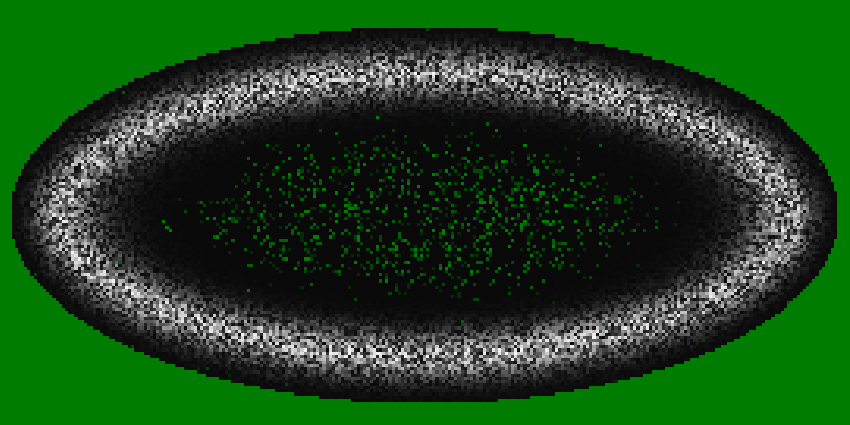
\includegraphics[width=\textwidth]{\Figures/Sblc/surface_cut.png}
        \label{fig:sblc:defaut:surface:fantôme}
    \end{subfigure}
    %
    \begin{subfigure}[b]{0.45\textwidth} 
        \caption{Résultat du SBLC sur le fantôme}
        \centering 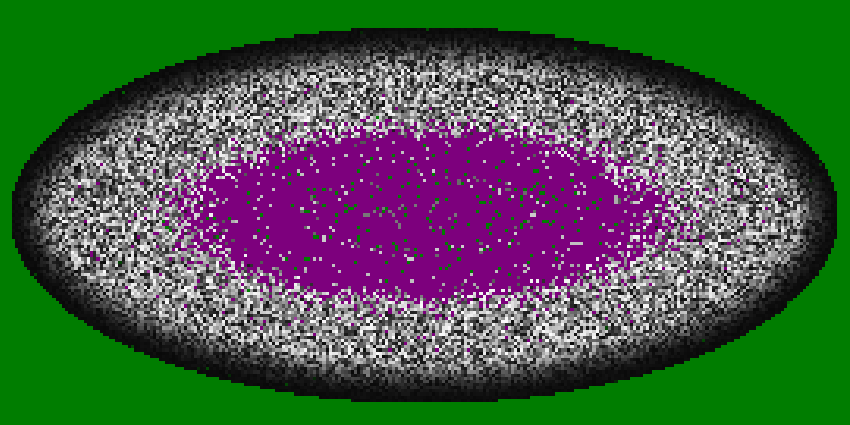
\includegraphics[width=\textwidth]{\Figures/Sblc/surface_corrected_cut.png}
        \label{fig:sblc:defaut:surface:application}
    \end{subfigure}
    %
    \caption{
        Modélisation de l'utilisation du SBLC sur un marquage de surface
        \newline
        Les voxels ayant une valeur de gris nulle ou supérieure à 4095 sont représentés respectivement en vert et en magenta.
        }
    \label{fig:sblc:defaut:surface}
\end{figure}

%%
%
A contrario, cette approche ne s'appliquant qu'à partir de l'épaisseur où le médian des valeurs de gris décroît, un signal présent uniquement dans la profondeur de l'échantillon ne serait que peu modifié par cette algorithme.
%
Il est donc impossible de compenser un défaut de marquages d'antigènes se trouvant dans les parties les plus profondes de l'échantillon.
%
Imaginons le marquage d'un antigène se trouvant dans l'hypothalamus d'un \pz{} à 5 dpf.
%
Cette région étant une des régions les plus profondes au sein d'un \pz{} à ce stade, un défaut de marquage ne pourrait pas être compensé, car il serait alors impossible de différencier le signal positif du bruit de fond se trouvant au niveau de la peau.
%
Ce défaut présente en soit une qualité car il permet de s'assurer qu'aucun signal faux-positif ne sera créé par l'algorithme  (voir Figure~\ref{fig:sblc:defaut:deep}).

\begin{figure}
    \centering
    \begin{subfigure}[b]{0.45\textwidth}
        
        \caption{Fantôme utilisé}
        \centering 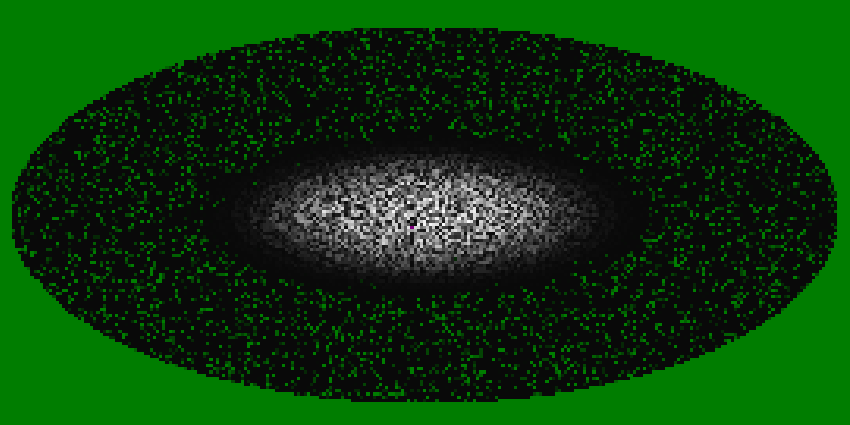
\includegraphics[width=\textwidth]{\Figures/Sblc/deep_cut.png}
        \label{fig:sblc:defaut:deep:application}
    \end{subfigure}
    %
    \begin{subfigure}[b]{0.45\textwidth} 
        \caption{Résultat du SBLC sur le fantôme}
        \centering 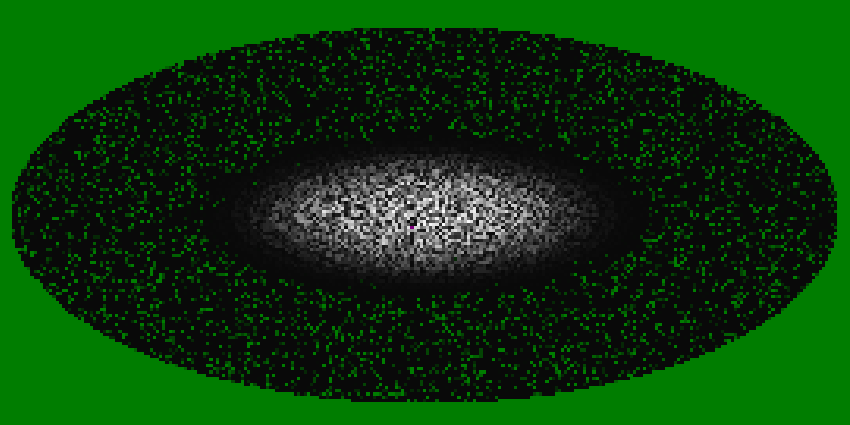
\includegraphics[width=\textwidth]{\Figures/Sblc/deep_corrected_cut.png}
        \label{fig:sblc:defaut:deep:application}
    \end{subfigure}
    %
    \caption{
        Modélisation de l'emploi du SBLC sur sur un marquage profond.
        \newline
        Les voxels ayant une valeur de gris nulle ou supérieure à 4095 sont représentés respectivement en vert et en magenta.
        }
    \label{fig:sblc:defaut:deep}
\end{figure}

%%
%
Par ailleurs, cet algorithme étant basé sur la multiplication de chaque couche par
un coefficient, un signal ayant complètement disparu ne pourra pas être récupéré (voir Figure~\ref{fig:sblc:defaut:surface0}). Les méthodes de clarification des larves de poisson zèbre restent donc insipensables. En leur abssence, le centre de la larve possède en effet des sign	aux trop faible pour que cet algorithme puisse compenser la perte trop forte de signal.
%
\begin{figure}
    \centering
    \begin{subfigure}[b]{0.45\textwidth}
        
        \caption{Fantôme utilisé}
        \centering 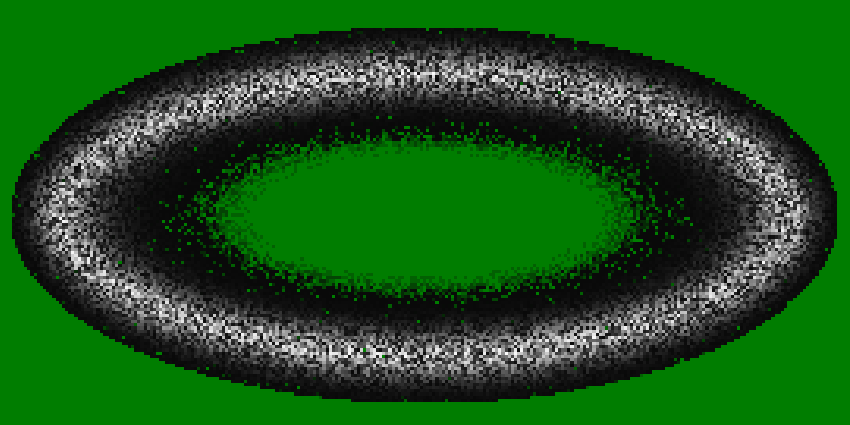
\includegraphics[width=\textwidth]{\Figures/Sblc/surface0_cut.png}
        \label{fig:sblc:defaut:surface0:application}
    \end{subfigure}
    %
    \begin{subfigure}[b]{0.45\textwidth} 
        \caption{Résultat du SBLC sur le fantôme}
        \centering 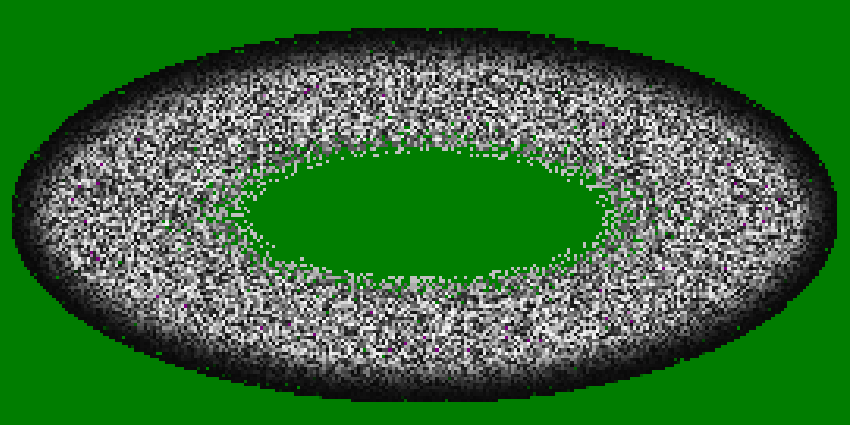
\includegraphics[width=\textwidth]{\Figures/Sblc/surface0_corrected_cut.png}
        \label{fig:sblc:defaut:surface0:application}
    \end{subfigure}
    %
    \caption{
        Modélisation de l'emploi du SBLC sur sur un marquage disparaisant avec la profondeur.
        \newline
        Les voxels ayant une valeur de gris nulle ou supérieure à 4095 sont représentés respectivement en vert et en magenta.
        }
    \label{fig:sblc:defaut:surface0}
\end{figure}

%%
%
Enfin, cette approche se basant sur un quotient entre valeur médiane maximale et valeur médiane pour la profondeur considérée, cette méthode permet de ne pas modifier un échantillon ayant été correctement marqué.
%
En effet, si les valeurs médianes ne sont que peu modifiées au fur et à mesure que l'on pénètre dans l'échantillon, le SBLC ne modifiera que très peu les valeurs de gris des couches concernant.

\end{document}
